\section{ICAE-Bench}
\label{sec:icae_bench}

\rcb{} is an interactive benchmark for from-scratch repository generation. This section defines a benchmark instance and describes its construction. The main design principle is to expose fuzzy requirements to the agent while evaluating the final repository through reliable behavioral evidence.

To do so, each task begins with a fuzzy PRD, allows clarification through a User Agent, and is finally scored by authoritative black-box cases that include both Public and Hidden cases. As shown in Figure~\ref{fig:framework}, there are mainly five stages: repository filtering, GroundPRD synthesis and test refactoring, PRD fuzzification, ultimate-image packaging, and artifact verification. This design gives \rcb{} realistic ambiguity, reproducible interaction, and language-agnostic evaluation. 

\begin{figure*}[t]
\centering
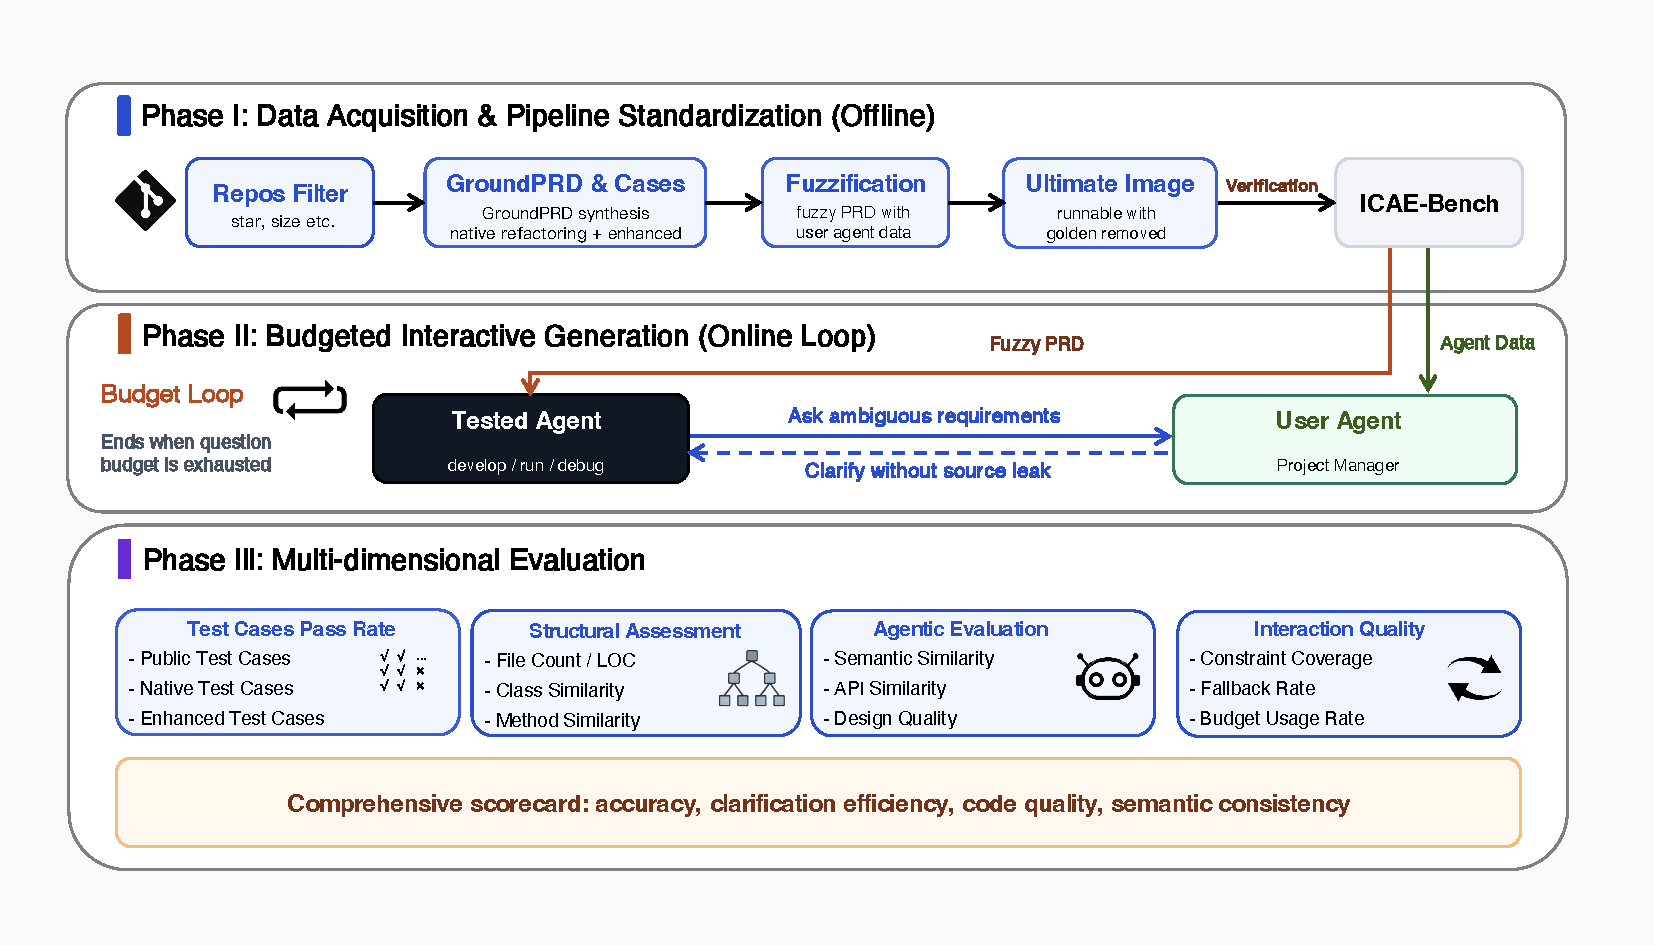
\includegraphics[width=0.94\textwidth]{figures/icae_bench_framework.pdf}
\caption{\textbf{\rcb{} framework.} A task begins with a fuzzy PRD and an ultimate image rather than a complete implementation contract. The coding agent can develop, execute, debug, and ask the User Agent for clarifications. Final repositories are evaluated using source-based Native and Enhanced black-box cases; the Public subset is also reported as a visibility-based view.}
\label{fig:framework}
\end{figure*}

\subsection{Benchmark Instance Definition}
\label{sec:task-definition}

Each benchmark instance separates what the coding agent initially sees, what it may recover through interaction, and what the evaluator uses as the behavioral target. Formally, an instance is
\begin{equation}
\mathcal{T}=(D_f,E,P,U,B),
\end{equation}
where $D_f$ is the fuzzy PRD and $E$ is the ultimate-image execution environment. The Public set $P$ contains illustrative Native cases recoverable through clarification, while $B$ contains all authoritative Native and Enhanced cases. User Agent Data $U$ stores omitted constraints, the complete input/output content of $P$, and the records that ground clarification responses. The coding agent observes $(D_f,E)$, queries the User Agent backed by $U$ under a fixed budget, and produces a repository $R$ that is evaluated against $B$.

For example, in a file-parser instance, $D_f$ requests the parser without enumerating all formats or edge cases; $P$ provides representative input/output examples when requested; and $B$ additionally tests unexposed malformed and boundary inputs. Thus, requirement exposure and behavioral evaluation remain distinct.

\begin{table}[htbp]
\centering
\caption{Roles of task components in \rcb{}.}
\label{tab:component-roles}
\small
\begin{adjustbox}{width=\linewidth, center}
\begin{tabular}{ll}
\toprule
Component & Role \\
\midrule
Fuzzy PRD ($D_f$) & Initial requirement \\
Ultimate image ($E$) & Execution environment \\
Public cases ($P$) & Visible or recoverable examples \\
User Agent Data ($U$) & Interaction oracle \\
Native + Enhanced cases ($B$) & Evaluation target \\
\bottomrule
\end{tabular}
\end{adjustbox}
\end{table}

\begin{table}[t]
\centering
\caption{Overview of the \rcb{} construction and evaluation pipeline.}
\label{tab:pipeline}
\small
\begin{tabular}{p{0.24\linewidth}p{0.65\linewidth}}
\toprule
Stage & Purpose \\
\midrule
Repository filtering & Keep repositories whose original tests pass in Docker. \\
GroundPRD and case construction & Synthesize requirements and refactor tests into authoritative black-box cases. \\
PRD fuzzification & Create the fuzzy PRD and grounded User Agent Data. \\
Ultimate-image packaging & Remove solution artifacts while retaining the provisioned runtime. \\
Artifact verification & Check semantic alignment and execution consistency across all task artifacts. \\
\bottomrule
\end{tabular}
\end{table}

\subsection{Benchmark Construction}
\label{sec:construction}

We summarize the construction process in five stages. Throughout the pipeline, GroundPRD, the fuzzy PRD, User Agent Data, and all behavioral cases must describe the same underlying task. First, we retain only repositories whose original tests pass in Docker so that every source task begins from stable, reproducible behavior. Second, we refactor the original tests into standardized black-box JSON cases and synthesize GroundPRD from the verified repository behavior. Third, we fuzzify GroundPRD into an ambiguous user-facing request plus structured User Agent Data, creating a controlled gap between what is initially visible and what can be recovered through interaction. Constraint selection spans API commitments, edge-case behavior, and architectural requirements, ensuring that fuzzification does not depend on a single ambiguity type. Fourth, we package each task into an ultimate image that removes golden code and hidden artifacts while preserving the runtime environment. Fifth, we validate semantic and execution consistency across the constructed artifacts. Stage-specific prompt templates are organized in the appendices.

\paragraph{Repository Selection and Test Refactoring}
We begin with real open-source repositories that provide runnable test suites. A repository is retained only if all of its original tests pass in a controlled Docker environment, ensuring that every benchmark task originates from stable, executable behavior. For each retained repository, we record its language, popularity, file count, golden-code lines of code (LOC), and an LLM-assisted assessment of test completeness, effectiveness, reliability, and readability.

We then transform the original tests into standardized black-box cases. Each leaf feature is represented by JSON inputs and expected outputs produced by a task-specific dispatcher running against the golden implementation. Only externally observable behavioral contracts are retained; language-specific exception details are normalized into repository-level error categories. A refactored case is accepted only after it executes successfully against the golden repository in its controlled environment. These retained cases form the Native suite; the separately synthesized Enhanced suite adds robustness coverage below. Together, they decouple evaluation from the original source layout, internal APIs, and implementation language.

\paragraph{GroundPRD Synthesis and Fuzzification}
Using the verified behavior, we construct GroundPRD as a natural-language specification of the required features and general software-engineering constraints. The construction agent selects approximately one or two representative Native cases per leaf feature for readability and embeds them in GroundPRD. These examples are mirrored exactly into the Public set; the remaining retained original-test cases stay Native and hidden. Selection is judgment-based rather than a fixed count or proportion. The examples make each feature concrete and establish the test-data format without exposing source code, original tests, internal APIs, or module structure.

Fuzzification converts GroundPRD into an incomplete product request while preserving the underlying task. The levels vary initial requirement exposure while retaining a common behavioral target: L1 is the least informative, L2 restores selected L1 ambiguity points, and L3 retains most of GroundPRD while hiding a limited set of details. In Fuzzy L1, GroundPRD is rewritten into a short PM-style request and selected API, edge-case, and architectural constraints are hidden. The complete Public examples and other omitted details are transferred into User Agent Data together with trigger keywords, grounded responses, contextual pointers, and a fallback response. Fuzzy L2 restores a subset of the ambiguity points hidden in L1. Fuzzy L3, the Easy setting, uses limited deletion and light ambiguity-oriented rewriting. The hierarchy is operational rather than a claim that ambiguity has a single universal scale; it controls how much task information is available before interaction. Because ambiguity points and their retrieval records are generated together, omitted information remains recoverable through sufficiently targeted questions.

\begin{figure}[t]
\centering
\begin{tikzpicture}[
  node distance=1.2mm,
  level/.style={draw, rounded corners=1.2pt, align=center, text width=0.82\linewidth, minimum height=5.2mm, font=\footnotesize},
  flow/.style={-{Latex[length=1.3mm]}, line width=0.5pt}
]
\node[level] (ground) {GroundPRD: complete specification};
\node[level, below=of ground] (l3) {Fuzzy L3: limited deletion and light rewriting};
\node[level, below=of l3] (l2) {Fuzzy L2: selected L1 ambiguity points restored};
\node[level, below=of l2] (l1) {Fuzzy L1: least initial requirement information};
\draw[flow] (l1) -- (l2);
\draw[flow] (l2) -- (l3);
\draw[flow] (l3) -- (ground);
\end{tikzpicture}
\caption{Initial-requirement hierarchy. Information available before interaction increases from Fuzzy L1 to GroundPRD, while the behavioral target remains fixed.}
\label{fig:prd-hierarchy}
\end{figure}

\paragraph{Enhanced Behavioral Cases}
Native cases preserve behavior covered by the original repository tests, but those tests may underrepresent difficult boundaries. We therefore synthesize Enhanced cases targeting boundary values, special constraints, stress behavior, and logic-specific corner cases. Enhanced cases must be disjoint from Native cases, and every synthesized case is executed against the golden implementation before acceptance. This adds robustness coverage without requiring generated repositories to reproduce the original implementation structure.

\paragraph{Ultimate Image Generation}
\label{sec:ultimate-image-generation}
The \emph{base image} is the official language-specific image downloaded from Docker Hub. We favor mainstream stable or LTS versions to maximize compatibility with real repositories while keeping the environment specification explicit and reproducible (Table~\ref{tab:image-versions}). To construct the \emph{ultimate image}, we run the golden repository successfully in the base image, install the dependencies needed by that repository, and then remove the golden code, original tests, and hidden construction artifacts. The result is a fully provisioned execution environment without solution artifacts: it retains the verified dependency stack while forcing the agent to rebuild the repository and its runnable interface from the exposed requirement information alone. For Kotlin, we use a Kotlin 1.9.25 environment built on Eclipse Temurin 17 and describe it generically to avoid deanonymizing any private image registry.

\begin{table}[htbp]
\centering
\caption{Language-specific execution environment images used for benchmark packaging.}
\label{tab:image-versions}
\small
\begin{adjustbox}{width=\linewidth, center}
\begin{tabular}{lll}
\toprule
Language & Runtime Version & Base Image \\
\midrule
C\# & .NET 8 & \texttt{mcr.microsoft.com/dotnet/sdk:8.0} \\
C++ & GCC 12 & \texttt{gcc:12} \\
Dart & Dart 3.5 & \texttt{dart:3.5} \\
Go & Go 1.22 & \texttt{golang:1.22} \\
Java & Java 17 & \texttt{eclipse-temurin:17} \\
JavaScript & Node 20 & \texttt{node:20} \\
TypeScript & Node 20 & \texttt{node:20} \\
Kotlin & Kotlin 1.9.25 & \texttt{Eclipse Temurin 17-based custom image} \\
PHP & PHP 8.2 & \texttt{php:8.2} \\
Python & Python 3.11 & \texttt{python:3.11} \\
Ruby & Ruby 3.2 & \texttt{ruby:3.2} \\
Rust & Rust 1.81 & \texttt{rust:1.81} \\
\bottomrule
\end{tabular}
\end{adjustbox}
\end{table}

\subsection{Artifact Verification}
\label{sec:artifact-verification}

Verification prevents benchmark-construction errors from being misattributed to coding agents. Repository-level executability is enforced upstream: retained golden repositories must pass their original and reconstructed Native cases, and every Enhanced case must pass against the golden implementation before acceptance.

We then establish GroundPRD correctness through iterative reconstruction in the ultimate image. Claude-Opus-4.8 implements each repository from GroundPRD, and we inspect failing Public or Native cases. We repair incorrect cases or revise an omitted or misstated contract, repeating the process until GroundPRD, Public examples, and Native cases are mutually consistent.

Finally, we verify that the fuzzy PRD and User Agent Data preserve the validated GroundPRD contract using two complementary checks. First, GPT-5.5 jointly compares the fuzzy PRD and User Agent Data with GroundPRD under a fixed rubric for semantic similarity, equivalence, and execution-contract risk. On \rcblite{}, Fuzzy L1 and L3 are equivalent to GroundPRD for all 50 repositories, with mean similarity scores of 0.952 and 0.942 and no case judged likely to fail the same tests. Second, black-box execution-equivalence checks validate the contract against the golden implementation. The two checks test semantic alignment and executable behavior, respectively. Prompts are provided in Appendices~\ref{appendix:fuzzy-prd-semantic} and~\ref{appendix:fuzzy-prd-easy-prompts}.

\paragraph{Generation Harness}
At evaluation time, the harness provisions a fresh container from the task image, exposes only the task-facing starter materials, and asks the coding agent to implement the repository entirely inside that container. A common interface integrates Claude Code and OpenHands while preserving their native editing and execution workflows. The prompt requires the agent to build its own execution adapter, use any Public examples recovered through interaction for self-checking, and make the repository reproducibly runnable. Final scoring replays the generated repository in a fresh container from the same image, so transient development-time actions count only when reflected in the delivered artifacts. The full instruction is included in Appendix~\ref{appendix:agent-task}.

\begin{table}[htbp]
\centering
\caption{Dataset statistics. Token lengths are computed over task documents and User Agent Data.}
\label{tab:dataset-statistics}
\begin{tabular}{lcc}
\toprule
\multirow{2}{*}{\textbf{Statistic}} & \multicolumn{2}{c}{\textbf{Count}} \\
\cmidrule(lr){2-3}
 & \textbf{\rcb{}} & \textbf{\rcblite{}} \\
\midrule
\textbf{GroundPRD Tokens} \\
~~~~- \textit{Maximum} & $43,990$ & $43,990$ \\
~~~~- \textit{Minimum} & $1,767$ & $1,767$ \\
~~~~- \textit{Average} & $6,764$ & $6,170$ \\
\midrule
\textbf{Fuzzy PRD Tokens} \\
~~~~- \textit{Maximum} & $367$ & $327$ \\
~~~~- \textit{Minimum} & $181$ & $226$ \\
~~~~- \textit{Average} & $276$ & $273$ \\
\midrule
\textbf{User Agent Data Tokens} \\
~~~~- \textit{Maximum} & $53,887$ & $53,887$ \\
~~~~- \textit{Minimum} & $515$ & $648$ \\
~~~~- \textit{Average} & $7,091$ & $6,945$ \\
\midrule
\textbf{Languages} & $12$ & $10$ \\
\midrule
\textbf{Total Tasks} & $480$ & $50$ \\
\bottomrule
\end{tabular}
\end{table}

\subsection{Benchmark Statistics}
\label{sec:statistics}

As shown in Table~\ref{tab:dataset-statistics} and Figure~\ref{fig:categories}, \rcb{} covers 12 programming languages: C\#, C++, Dart, Go, Java, JavaScript, Kotlin, PHP, Python, Ruby, Rust, and TypeScript. The full benchmark contains 40 tasks per language. \rcblite{} is selected from \rcb{} by prioritizing smaller repositories according to golden-code LOC, making it suitable for rapid ablations and framework comparisons. Figure~\ref{fig:repo_loc} shows the full benchmark's golden-code LOC distribution.

\paragraph{Golden LOC.}
Maximum: $2,918,810$ / $1,509$; minimum: $318$ / $318$; average: $35,533$ / $979$ for \rcb{} / \rcblite{}, respectively.

\paragraph{Golden File Count.}
Maximum: $17,488$ / $61$; minimum: $4$ / $4$; average: $258$ / $17$ for \rcb{} / \rcblite{}, respectively.

\begin{figure}[t]
\centering
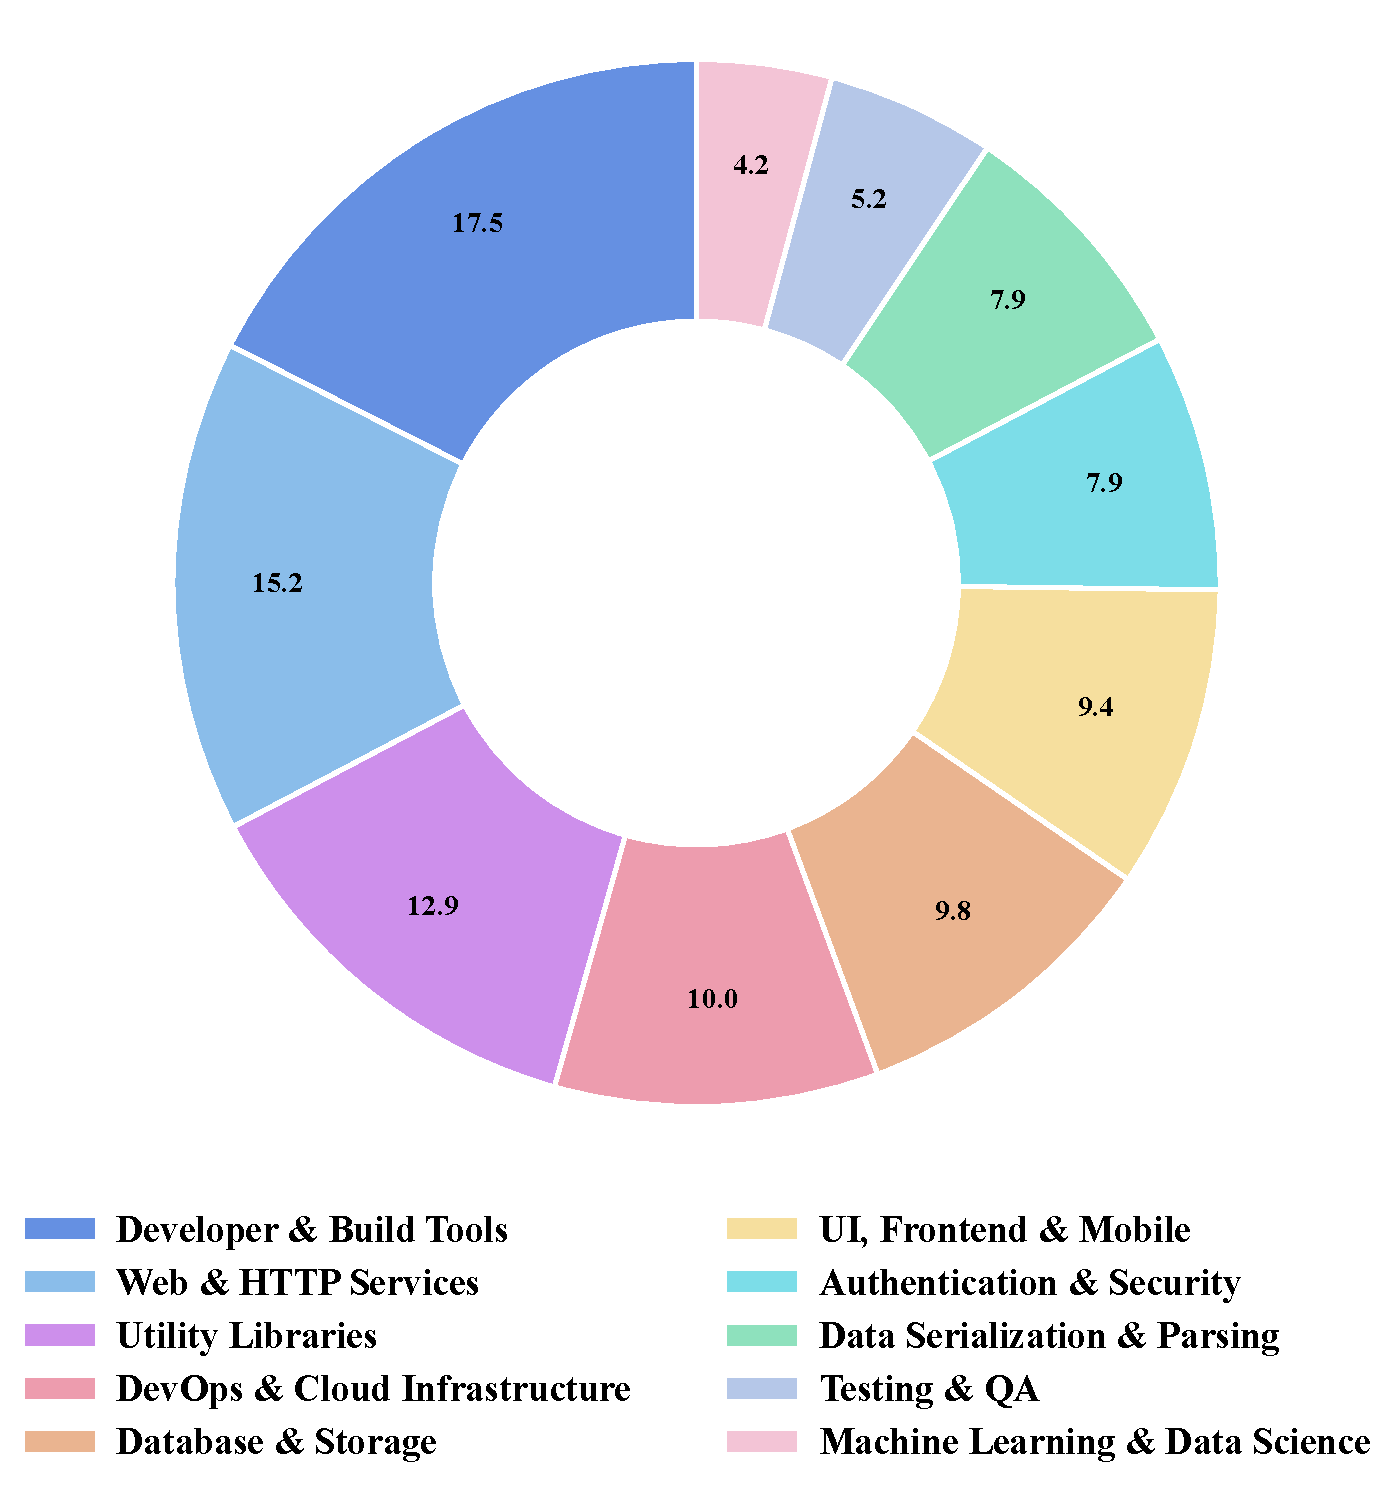
\includegraphics[width=\linewidth]{figures/icae_bench_domain_distribution.pdf}
\caption{Task category distribution in \rcb{} (total=480).}
\label{fig:categories}
\end{figure}

\begin{figure}[htbp]
\centering
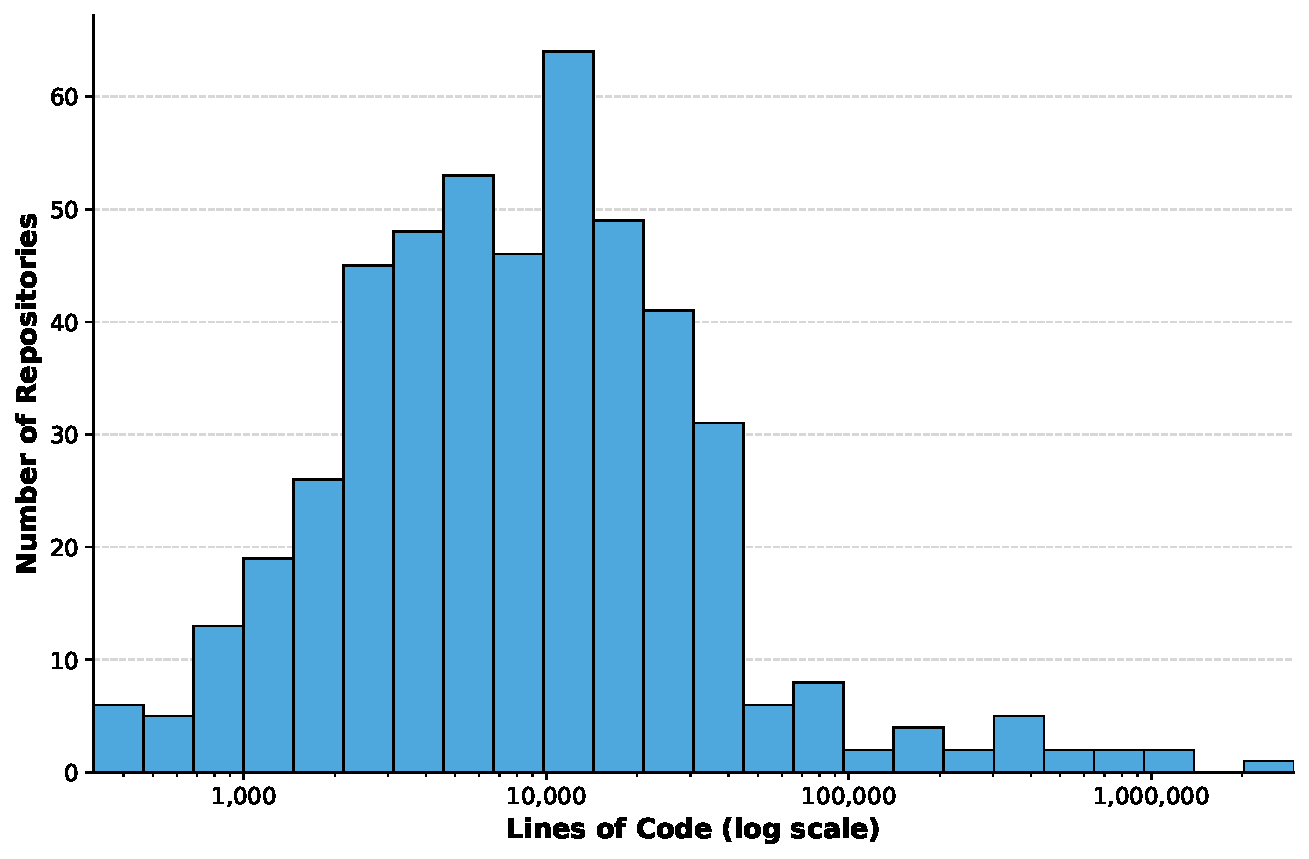
\includegraphics[width=0.7\linewidth]{figures/repo_loc_histogram.pdf}
\caption{Task golden-code LOC distribution in \rcb{} (total=480).}
\label{fig:repo_loc}
\end{figure}

\subsection{Interactive User Agent}
\label{sec:user-agent}

The User Agent is a model-based router that simulates a strict product stakeholder. Our default configuration uses DeepSeek-V3.2 and a budget of 16 queries. The coding agent sends a task identifier and one natural-language question to an HTTP endpoint; the server loads that task's User Agent Data, invokes the router, and returns a natural-language reply together with the remaining budget. Each reply addresses at most three matched technical points, after which the coding agent may issue the next query. The full request format and initialization prompt are provided in Appendices~\ref{appendix:suffix} and~\ref{appendix:user-agent}.

Routing is restricted to benchmark-authored records. During fuzzification, each omitted ambiguity point is assigned an identifier, semantically equivalent trigger phrases, a grounded response, and optional context pointers; omitted Public examples and a fixed fallback response are stored in the same task data. For each query, the router may return only responses associated with matched records or the fallback. Its structured internal log records matched constraint identifiers, interface-alignment events, and fallback use.

This protocol limits leakage at three boundaries. The User Agent receives no golden source code, original tests, repository identity, or hidden evaluation cases; its task knowledge is limited to the generated records. The coding agent receives only the router's natural-language reply, not the records or internal log. Each tested agent develops in an isolated Docker container without authoritative cases; those cases are injected only into a fresh evaluation container after generation. Thus, interaction can reveal omitted requirements and Public examples, but not solution artifacts or hidden test contents.


\subsection{Evaluation Metrics}
\label{sec:metrics}

\paragraph{Functional Correctness}
Functional correctness is the primary measure of whether a generated repository implements the required externally observable behavior. We organize cases along two orthogonal axes. By source, \emph{Native} cases are transformed from original repository tests, whereas \emph{Enhanced} cases add synthesized robustness coverage. By visibility, \emph{Public} cases are exposed in GroundPRD and \emph{Hidden} cases are all remaining cases. Public is a subset of Native, so $\mathrm{Hidden}=(\mathrm{Native}\cup\mathrm{Enhanced})\setminus\mathrm{Public}$; Public/Hidden are visibility partitions, whereas Native/Enhanced are source partitions. Fuzzy L1/L2 omit Public cases from the initial PRD, but they remain recoverable through interaction. Tables~\ref{tab:main-results-full} and~\ref{tab:main-results-lite} report Public, Native, and Enhanced views. \emph{Overall} is the case-level pass rate over all Native and Enhanced cases, computed as $(\#\text{passed Native}+\#\text{passed Enhanced})/(\#\text{Native}+\#\text{Enhanced})$. Evaluation is host-verified: a fresh container receives the authoritative cases, runs the agent-produced entry point, and returns outputs for host-side comparison.

\paragraph{Agentic Evaluation}
Functional tests cannot distinguish a narrowly hard-coded solution from a maintainable repository. We therefore use static critic-model review over the generated and golden source trees. Semantic similarity measures alignment of behavior and abstractions; API similarity compares importable types, functions, names, signatures, and coverage; and design quality assesses the generated repository's architecture, including separation of core logic from the execution adapter. These independent scores diagnose behavioral breadth, interface fidelity, and engineering quality, respectively. The critic prompt is included in Appendix~\ref{appendix:critic}.

\paragraph{Structural Assessment}
Repository-scale failures may be hidden by case-level pass rates. We therefore compare generated and golden repositories using file-count and LOC ratios plus class, method, and namespace/package similarities. These diagnostics reveal under-building, over-building, or collapsing a multi-module project into a monolithic adapter; they do not reward literal reproduction of the golden implementation.

\paragraph{Interaction Quality}
Interaction metrics measure whether an agent retrieves relevant hidden requirements efficiently. From the router logs, let $C$ be the hidden constraint identifiers and $H$ the unique identifiers matched at least once. Constraint coverage is $|H|/|C|$; fallback rate is the fraction of queries matching no grounded record; and budget usage is the issued-query count divided by the allowed budget. We macro-average task-level rates so tasks with more constraints do not dominate.

Pass rates, agentic scores, structural similarities, and constraint coverage are higher-is-better within their respective dimensions; fallback rate is lower-is-better, and budget usage is descriptive. File-count and LOC ratios may exceed 100\%; values near 100\% indicate similar scale, not necessarily better quality.
